\section{System Architecture}\label{sec:system_deployment}

\subsection{Out-of-Network Recommendations}
%Out of Network Recommendations serve as one of several initial ranking sources for the LinkedIn Homepage Feed. When a member accesses the feed, a request is sent from the front end to the feed service, which then delegates to several first pass rankers, including the feed-OON mid tier (a.k.a. interest discovery), tasked with discovering interests. This service retrieves the top-K most suitable items for the member using a lucene-based index.

%As shown in Figure \ref{fig:OONArchitecture}, each member query triggers an embedding-based search across all eligible item embeddings, followed by a first-layer (L1) ranking model to select the top-K items. These are then forwarded to the feed service and undergo a second, more complex layer (L2) ranking model for member viewing.

%{\systemname} is designed to run online model-based retrieval algorithms, aiming to surpass our existing benchmarks: (1) dot-product based EBR, and (2) FAISS-IVFPQ, both integrated within LinkedIn's lucene systems.


Out of Network Recommendations is one of the many sources (first pass rankers) of Linkedin Homepage Feed. When a member visits Linkedin feed, a request is triggered from the front end and sent to feed service. Feed service passes this request to many first pass rankers including feed-OON mid tier (a.k.a. interest discovery). This service is responsible for retrieving the top-K most eligible items for the member to send back to feed. Today, the underlying index used for retrieval is a lucene based index. 
The runtime of the query of OON is depicted at Figure \ref{fig:OONArchitecture}. For every member query, a embedding based search is performed across all eligible item embeddings, followed by a layer 1 (L1) ranking model, which decides top-K items. 
These are then sent to feed service and ranked by more sophisticated layer 2 (L2) ranking model for members consumption.
{\systemname} aims to provide an online service to run model based retrieval algorithms that can outperform our baselines: (1) dot-product based EBR, and (2) FAISS-IVFPQ, which is supported at Linkedin for lucene systems. 

%Being a new product that was tested on Linkedin feed, OON heavily relies on an offline inference framework to run embedding based retrieval.
%The top-K items are then stored on a cloud based storage for online lookup. During online query, this top-K is retrieved, gets further filtered by lucene term based product rules, 

\begin{figure}
  \centering
  \vspace{-4pt}
  \begin{adjustbox}{max size={\linewidth}{\textheight}}
  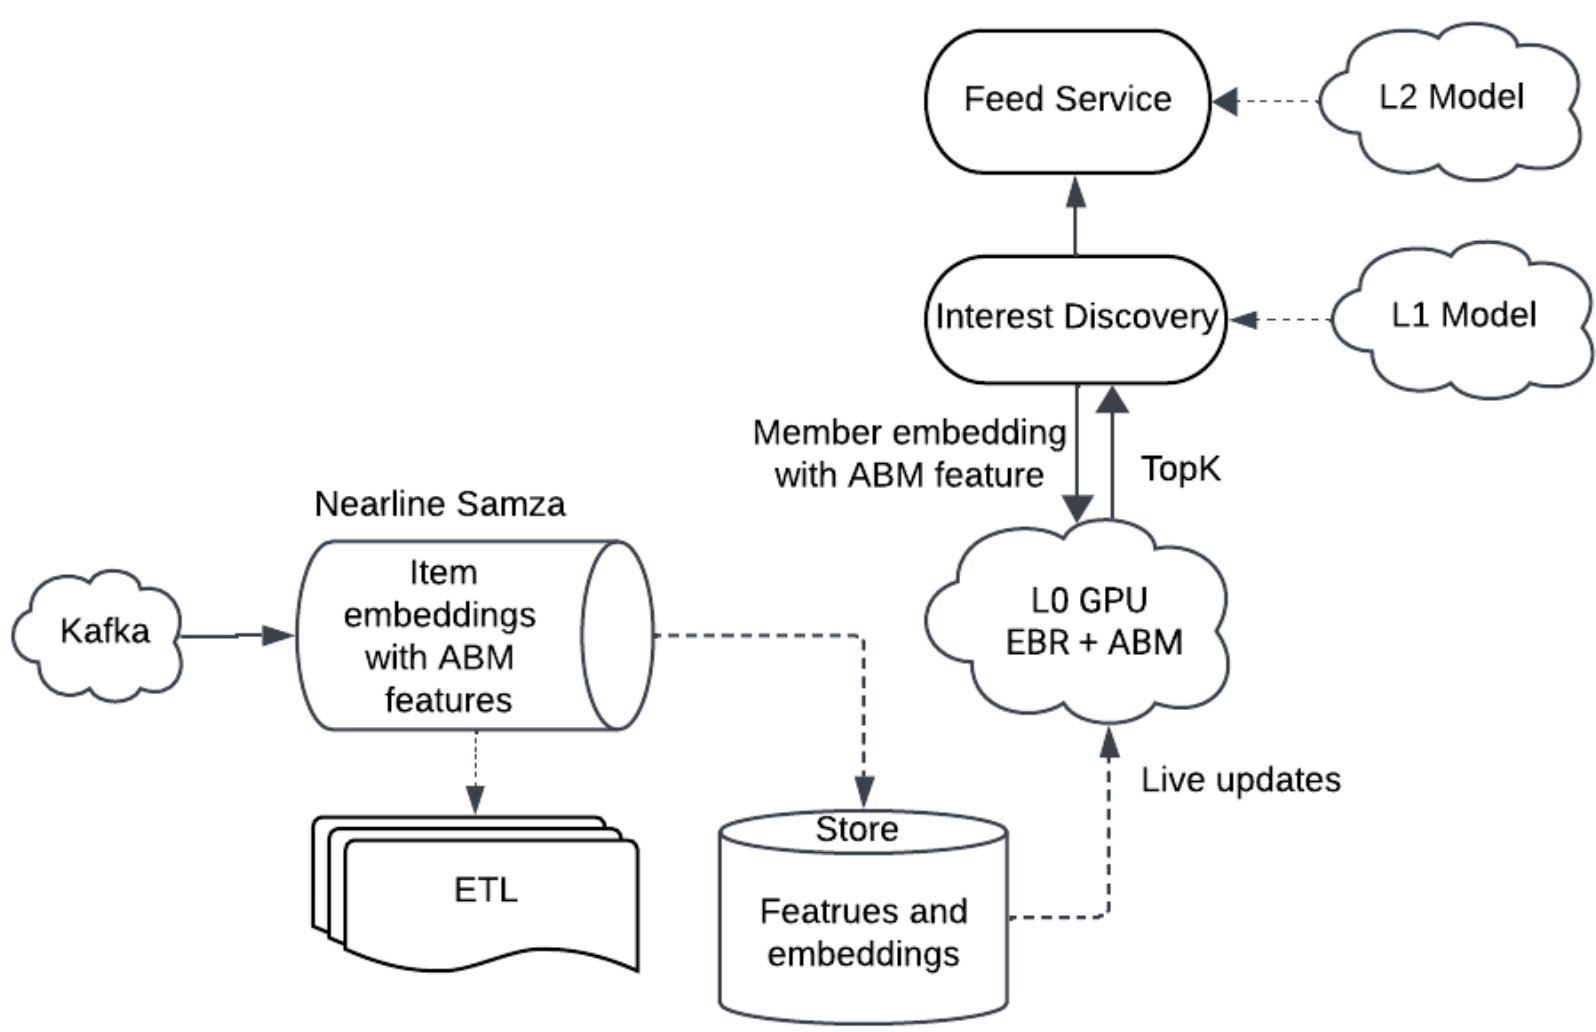
\includegraphics{figures/Feed_OON_small.png}
  \end{adjustbox}
  \caption{\small Feed OON Architechture.}
  \label{fig:OONArchitecture}
  \vspace{-12pt}
\end{figure}

As shown in the figure, interest-discovery will call model-cloud-L0 to fetch candidate items for the member. Model-cloud-L0 hosts the RAR model that does (1) item attribute-based filtering (2) embedding based retrieval with ranking using model. The model consists of the item embeddings, features needed for filtering and the trained model weights.  Item embeddings are generated on a nearline fashion as and when a document is created at Linkedin so as to keep the index up to date. The filters required for filtering are also ingested nearline. 


\subsection{ML Infra Architecture}\label{sec:MLinfra}
We enhance Model Cloud, our hosted solution for serving model inferences, to support retrieval as ranking as shown in Figure 5.
\subsubsection{Retriever}
This component performs attribute-based filtering and embedding-based retrieval of the top-k documents for a query. At startup, retriever initializes with the retrieval model and bootstrapped data. Its framework-agnostic design allows easy extension to any framework, such as Torch or TensorFlow. AI engineers can experiment with new methods by developing and deploying corresponding models to this system.

%This component is responsible for attribute based filtering and embedding based retrieval of the top-k documents for a given query. At startup, retriever initializes itself with the retrieval model and bootstrapped data. Being framework agnostic makes this component easy to extend to any modeling framework such as Torch, TensorFlow. Plug and Play:  AI Engineers can experiment with innovative approaches such as the ones discussed in this paper by simply developing a corresponding model and deploying to this system.
\subsubsection{Ingestor}
Model-based retrieval requires the entire document corpus to reside in GPU memory for low latency. To provide fresh results, this corpus must be updated near real-time (nearline). Several following components work together to achieve this functionality.
%Model based retrieval and its low-latency requires the entire corpus of documents live in GPU memory. To serve fresh results, this corpus of documents must also be updated near real time (nearline). We have the following components working together to achieve this functionality.

\textit{Index Store:}
%Features such as attributes and embeddings are delivered by offline data sources and nearline data streams. We leverage Apache Beam in our feature delivery system to join and transform feature data for the whole corpus of documents. Offline, the entire corpus is batch-pushed to a Venice Store. Nearline, updates to the corpus are written to the same Venice Store.
Attributes and embeddings come from offline sources and nearline data streams. We use Apache Beam to join and transform feature data for the entire document corpus. Offline, the full corpus is batch-pushed to a Venice Store. Nearline updates are also written to this Venice Store.

\textit{Updator:}
Updator subscribes to the Index Store's Change-Data-Capture (CDC) Stream. As the feature data gets batch pushed and live updated, the Updator gets notified to further process them and write to the model.

\textit{Bootstrapper:}
At startup, the Ingestor bootstraps from the Venice CDC client by replaying all data from the beginning. The entire data corpus is transformed into the required format and copied to the GPU. To minimize bootstrapping time, we regularly compact the bootstrap data and store a snapshot on disk for a fast warm start.
%When retrieval service starts up, Ingestor bootstraps from the Venice CDC client by replaying all the data from the beginning of time. With the entire corpus of data in memory, it is transformed into the required format and copied to the GPU. We ensure that the bootstrap data is compacted regularly to keep the bootstrapping time to a minimum. We also store a snapshot on disk to enable fast warm start of the service.
\subsubsection{Service}
To meet our performance needs, we avoid the latency and unpredictability of managed, garbage-collected languages. We also minimize network hops, data copies, and transformations. Our Model Cloud L0 service is written in a native language with minimal data transformations. User queries from the L0 client land directly on our service, ensuring we meet latency requirements.
%To meet the scale and performance requirements of our members, we cannot afford to take on the latency overhead and unpredictability that comes with managed, garbage-collected languages. Additionally, network hops, data copies and data transformations should be kept at a required-minimum. Keeping this in mind, our Model Cloud L0 service is written in a native language with minimum to no data transformations. User's query from the L0 client lands directly on our service. This way we are able to meet the latency requirements of our users.
\begin{figure}
    \centering
    \vspace{-4pt}
    \begin{adjustbox}{max size={\linewidth}{\textheight}}
        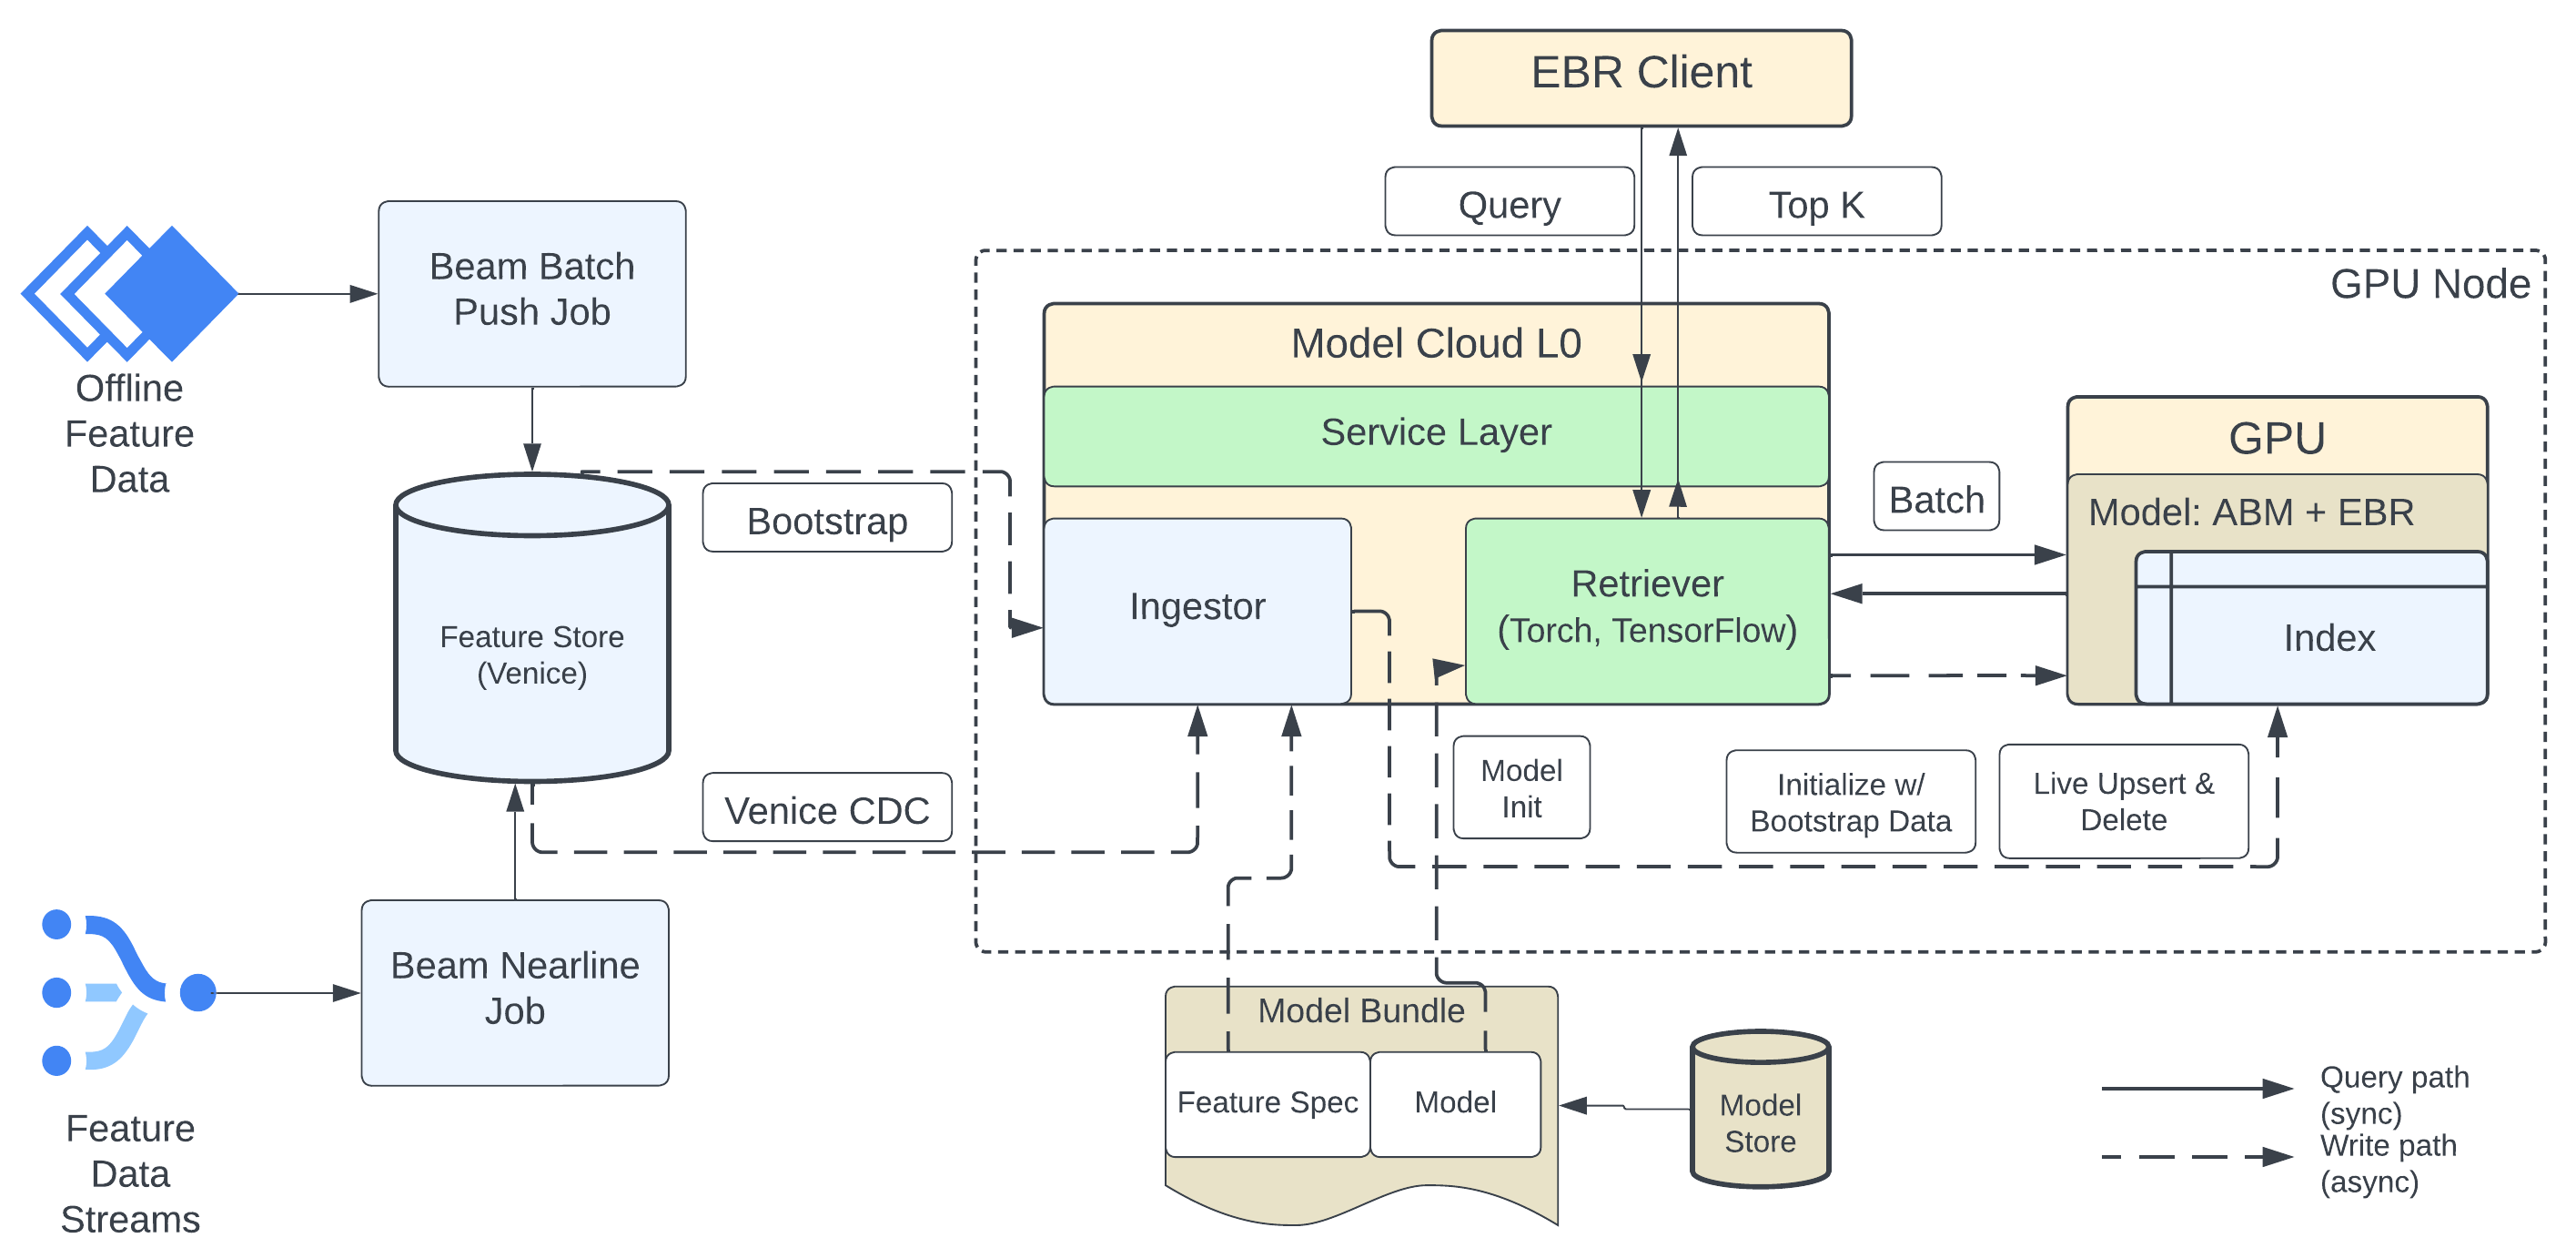
\includegraphics{figures/Model_cloud.png}
    \end{adjustbox}
    \caption{\small Model Cloud {\systemname} Architecture}
    \label{fig:enter-label}
    \vspace{-14pt}
\end{figure}

\subsection{Model Live Update}\label{sec:live_update}
Live Update Ingestor subscribes to Venice CDC~\cite{veniceDB} from the bootstrapped offset, classifying changes into upserts and deletes, then transforming and copying them to the GPU.

The system's effectiveness depends on the quality of the document index, which must remain fresh. This can be done by either regularly rebuilding the index or updating it in near-real-time via a data change stream. We chose the latter for two reasons: it keeps the corpus current, reflecting changes within seconds, and it's more efficient, avoiding the cost of rebuilding and replacing the entire index. To implement this, we modified the PyTorch model to expose Upsert and Delete APIs, ensuring safe and efficient concurrent index updates during inference. Techniques used include pre-allocating larger tensors, using a high-water mark to track the working set, and making thread-safe in-memory tensor manipulations with minimal data access serialization. These methods ensure that modifications have minimal to no impact on the inference path, as detailed in the Model Inference Benchmarking section.
%Live Update Ingestor subscribes to Venice CDC from the bootstrapped offset. Changes are classified into upserts and deletes, transformed into the correct format, and copied to the GPU.

%Even though the system functions to surface the best candidates for ranking, its effectiveness is bounded by the quality of the underlying document index. In that aspect, it is essential to keep the index fresh by applying the changes in the underlying data. This could be achieved by either rebuilding the index in regular intervals or constantly updating it in near-real-time with changes pushed through a data change stream. We opted to implement the latter approach as its benefits are twofold. It offers a more current corpus as changes are typically reflected within a few seconds of their creation. Additionally, it is more efficient, as it avoids the cost associated with rebuilding the entire index and replacing a set of older ones. To follow this approach, we modified the PyTorch model to expose Upsert and Delete APIs and implemented them carefully so that the concurrent modifications to the index during the inference can be done safely and efficiently. We used techniques like pre-allocating larger tensors than the initial index requires, using high-water-mark to mark the working set of the tensors and making thread-safe in-memory manipulations on the tensors with minimal data access serializations. These details resulted in modifications having minimal to no impact on the inference path, as described in the Model Inference Benchmarking section.

\subsection{Inference on Native Stack}
We built a native serving system as we made performance and efficiency our top priorities. To serve the PyTorch model in this system, we had to convert it to a compatible format. There are a few alternatives for this purpose such as TorchScipt and torch.export. PyTorch supports two execution modes: eager mode and graph mode. Optimal performance is achieved by executing everything in graph mode as the operators are first synthesized into a graph, which are compiled and executed as a whole. We picked TorchScript for our initial implementation to execute the model in graph mode. However, by doing so we traded off the performance with ease of development. TorchScript is a subset of Python and comes up with some constraints. It requires static typing and does not support things like exceptions and data-dependent control flows. We found executing this conversion quite challenging and concluded that it should be a part of the model development rather than an afterthought. We also decided to pursue other options which are deemed to be more recent technologies such as torch.export.
